% $Id: loaders.tex 9832 2022-02-11 18:23:40Z mskala $

%
% Firmware loader and image builder
% Copyright (C) 2022  Matthew Skala
%
% This program is free software: you can redistribute it and/or modify
% it under the terms of the GNU General Public License as published by
% the Free Software Foundation, version 3.
%
% This program is distributed in the hope that it will be useful,
% but WITHOUT ANY WARRANTY; without even the implied warranty of
% MERCHANTABILITY or FITNESS FOR A PARTICULAR PURPOSE.  See the
% GNU General Public License for more details.
%
% You should have received a copy of the GNU General Public License
% along with this program.  If not, see <http://www.gnu.org/licenses/>.
%
% Matthew Skala
% https://northcoastsynthesis.com/
% mskala@northcoastsynthesis.com
%

\chapter{Loader and image builder (loader.s, image.s)}

This chapter describes the loader, with which the Gracious Host can rewrite
its own firmware; as well as the file format of loadable firmware files, and
how the build system gets the firmware into that format.  Other code
modules, notably the FAT driver in usbmass.s, are responsible for copying
the firmware image file into the SRAM chip; then the loader described here
does the reprogramming of the flash memory.

\section{Firmware update process}

It was a design goal for the Gracious Host that it should be able to update
its own firmware by loading a file from a USB mass storage device.  That
presented serious challenges for the design of the firmware.  If using
Microchip's C-language drivers for communicating with USB mass storage and
reading files from a FAT filesystem, the code just to read the new
firmware image would fill well over half the program memory capacity of the
microcontroller.  If that code were subject to update, the obvious way to do
it would be to read the entire new firmware into unused space in program
memory while leaving the old firmware intact, then either just switch to it
(accepting that the new firmware would have to be at a different address
from the old), or use a small stub to move the new code to its final
address, overwriting the old firmware including the old USB and FAT drivers. 
Either case requires at some point having two entire firmware packages in
program memory at once, which is impossible if they each consume more than
half the space.  Even if the ``old firmware'' were stripped down to just the
loader code, the loader code itself being bigger than half the program
memory poses a problem.

Another alternative might be to make the loader code \emph{not subject to
update}.  It would just remain fixed for all time after initial programming
of the chip, and any new firmware that might be loaded would be only
whatever parts were not needed to run the firmware update, safely rewritable
during the update process.  That is how most commonly-available boot loader
code works, including the example USB boot loader code for this chip
provided by the Microchip corporation.  The loader does not rewrite itself. 
But that approach precludes ever fixing or meaningfully changing the loader
code, which would be a large fraction of all the code on the chip.  It would
be a major compromise to the goal of allowing modification.

The Gracious Host uses another approach, supported by additional hardware in
the shape of the 128K SRAM chip.  To run a firmware update the old firmware,
including the large USB and FAT drivers, reads the new firmware image into
the SRAM, not into program memory.  Then it runs a small loader
process, whose source code is in the file loader.s.  The loader takes its
instructions from the image in the SRAM, not from the USB device; so it does
not need to run the USB and FAT drivers and can safely overwrite them.  It
only needs to communicate with the SRAM chip over SPI, and the
microcontroller's built-in flash memory hardware, each of which is a much
simpler interface than USB.

The firmware includes two copies of the loader, which in consequence must be
written with even more care than usual to keep the code small and
self-contained.  The linker puts one copy at the bottom of memory (lowest
addresses available after the interrupt table) and one at the top (highest
addresses available before the special non-reprogrammable last page).  See
the memory map in Figure~\ref{fig:memory-map}.

\begin{figure}
  {\centering
  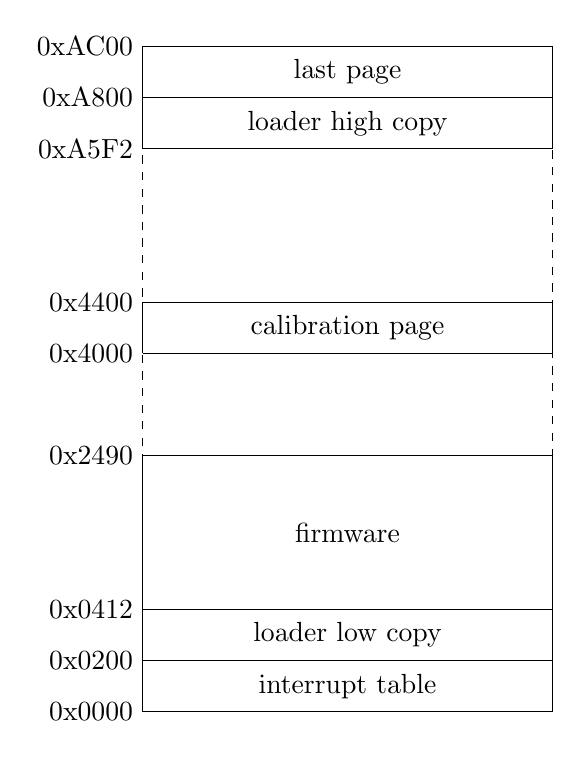
\begin{tikzpicture}[scale=1.3]
    \draw[dashed] (0,0) rectangle (4.0,6.5);
    \draw (0,0) -- (0,2.5);
    \draw (4.0,0) -- (4.0,2.5);
    \draw (0,3.5) -- (0,4.0);
    \draw (4.0,3.5) -- (4.0,4.0);
    \draw (0,5.5) -- (0,6.5);
    \draw (4.0,5.5) -- (4.0,6.5);
    \foreach \x/\y in {0x0000/0,0x0200/0.5,0x0412/1.0,0x2490/2.5,0x4000/3.5,
        0x4400/4.0,0xA5F2/5.5,0xA800/6.0,0xAC00/6.5} {
      \draw (0,\y) -- (4.0,\y);
      \node[anchor=east] at (0,\y) {\x};
    }
    \node at (2.0,0.25) {interrupt table};
    \node at (2.0,0.75) {loader low copy};
    \node at (2.0,1.75) {firmware};
    \node at (2.0,3.75) {calibration page};
    \node at (2.0,5.75) {loader high copy};
    \node at (2.0,6.25) {last page};
  \end{tikzpicture}\par}
  \caption{Program memory map (typical; exact addresses will vary; not to
    scale).}\label{fig:memory-map}
\end{figure}

The low copy runs first.  It is expected to write whatever parts of the new
firmware go into the top half of program memory -- including the new
firmware's high copy of the loader code.  The new loader code could
concievably differ from the old firmware's loader code, although new
firmware needs to be aware of any potential compatibility issues here.  Then
after the top half of the program memory space has been written, the new
firmware image directs the old loader, low copy, to jump to the newly
written high copy of the new loader.  That loader code continues the
operation of rewriting the program memory, filling in whatever parts of the
new firmware go into the low half of the
space.  At the end of the process, the entire rewritable portion of program
memory has, at least potentially, been rewritten.  All parts of the old
firmware, including the loader but excluding the non-reprogrammable last
page, can be replaced by the new firmware, despite the new firmware possibly
being the entire size of program memory.

I designed this process based on the observation that Microchip's C code
required something like 50K of program memory space just for a minimal USB
and FAT driver.  I expected that I could shrink the USB and FAT code
somewhat by replacing it with hand-optimized assembly language, but that I
would also have to add a significant amount of code to implement all the
rest of the things the firmware does beyond just reading files from a USB
mass storage device; so I could not be confident of making the entire
firmware \emph{less than half} the 64K capacity of the microcontroller. 
Being unable to fit two copies of the firmware in program memory at once was
the impetus for adding the SRAM chip.

In the event, my efforts to keep the code small were much more successful
than expected.  As of this writing the basically complete firmware fills
only about 17K of program memory, significantly less than half the available
space.  In principle, a scheme that read the entire new firmware into unused
space in program memory and then went from there, without needing the SRAM
chip, would probably work, and would save the cost of the additional
hardware.  However, the SRAM chip scheme is already implemented and it
works.  Writing and debugging a completely different loader system (as well
as changing the hardware design, even if only so far as just deciding not to
install the SRAM chip on the existing circuit board layout) seems like it
would be wasted effort; having the SRAM chip available for other purposes
seems to be of some value; and allowing for possible future firmware to use
all of program memory even if the current version uses less than half, seems
valuable too.  My plan is to stick with this design even if it seems
over-engineered for the current version of the standard firmware.

\section{Double assembly}

In order to help make sure that the low and high copies of the loader
function identically, they are both assembled from the same source file. 
Rules in the Makefile assemble the two object files loader-lo.o and
loader-hi.o from loader.s.  The symbol loader\_high\_copy is defined to 1 by
an assembler command-line option when assembling loader-hi.o, for use by
conditional assembly directives inside the source file in places where the
two copies need to differ.

The high copy should be located such that its text section (the binary
instructions that are the main output of the assembler) \emph{ends} with the
instruction at 0xA7FE, which is the last instruction before the reserved
final page of program memory.  The toolchain supports forcing a section to
start at a given address, but not easily forcing a section to end at a given
address.  (It might be possible with some trickery in the linker script, but
at the time I implemented this part, I was trying to avoid using a custom
linker script.) So in order to make the high copy end immediately before the
final page, more code in the Makefile reads loader-lo.o, finds the length of
the text section, and uses a Perl script named mkloaddr to write
loader-addr.inc, which contains the .section directive that will be used for
assembling the high copy to put it in the right place.

The mkloaddr utility finds the difference between the addresses marked by
the labels loader\_start and loader\_end in loader-lo.o.  It also applies an
adjustment defined by the loader\_delta label, if any.  This label can be
defined in the source code if there are any small differences between the
two versions of the loader that could affect the length.  It is measured in
address units, two units per 24-bit instruction, and it should be positive
if the high copy is longer, negative if the high copy is shorter.

Having two object files built from the same source unfortunately confuses
Microchip's debugger and I don't have a good solution to that, but it seems
to work reasonably well as long as execution stays in the low copy, and most
debugging tasks can be accomplished using only the low copy.

\section{Format of the image file}

Firmware to be loaded by the module needs to be formatted into an
\emph{image file}, so called because it is an exact image of the SRAM
contents at the start of the program memory writing process.  The standard
name for the firmware image file is firmware.frm (FIRMWARE.FRM in the
convention of the DOS FAT filesystem, which is case-insensitive but usually
writes filenames in all caps).  The image file can be up to 128K, the size
of the SRAM, though because there is only about 64K of program memory, it is
unlikely that an image file much larger than 64K would be useful.

The first 256 (0x0100) bytes of the image file are not used by the loader,
but are normally expected to be included in CRC checks.  This would be a
good place to include a human-readable identification of what the file is, a
copyright notice, and so on.

Starting at offset 0x0100, the main body of the file consists of a linked
list of \emph{loader records}, which are commands to the loader.  The loader
starts with the record at 0x0100 and then follows the links, executing each
command until one causes it to stop.

The first four bytes of each record are an identifier of the record type
(one byte, always an ASCII uppercase alphabetic character), and then a
24-bit pointer to the next record, as offset from the start of the file. 
Record types are referred to by their identifying letter, like
\emph{B-records} and \emph{C-records}.  After that header shared by all
record types, there may be other fields defined by the particular record
type, as discussed below.  Note that the next-record pointer is stored
\emph{unaligned} and \emph{little endian}; and the high byte of the pointer
is expected to always be equal to 0 or 1 because anything else would point
outside the 128K SRAM address space.  Notwithstanding the exception of the
24-bit next-record pointer, other fields in loader records of 16 bits or
more, and the records themselves, are expected to be 16-bit aligned.

Extra bytes of padding between and after loader records is allowed, a
fact used in the standard firmware's image generator to get around
toolchain limitations, as discussed in the section on image.s below.  In
principle, loader records need not even be arranged in sequential order
within the file; the loader just follows the link fields to successive
records wherever they are.

\section{SRAM simulation and common macros}

Debugging the loader works well on real hardware with a real SRAM chip; the
SRAM is tolerant of long gaps in the timing, as might be caused by
single-stepping the processor.  Debugging the loader code in the PIC24F
simulator works less well because there is nothing connected to the
simulated SPI port; the firmware tries to send commands to the SRAM chip but
never gets any responses.  So to allow for debugging in the simulator, there
is support in loader.s for building a small image file into program memory
and reading that instead of the SRAM.  If SIMULATE\_SRAM is defined in
config.inc, the loader will read SRAM data from program memory instead of
attempting to connect to the SRAM chip.

All communication with the SRAM in loader.s is done through seven macros:
assert\_cs2, retract\_cs2, mov\_to\_spi1buf, clr\_spi1buf, setm\_spi1buf,
mov\_b\_from\_spi1buf, and btst\_srxmpt.  When simulation is \emph{not}
enabled, each of these is defined to assemble a single instruction that
interacts with a relevant hardware register.  When SIMULATE\_SRAM is
defined, they instead implement a minimal simulation of the SRAM chip's
communication protocol, supporting only the read command.  There are a
couple of static variables and support subroutines assembled and used by
these macros.

The data stored in the the simulated SRAM is a manually-constructed image
file assembled at the label sram\_data.  It can of course be edited as
needed for a given debugging task, but the version in the source code is an
assortment of records intended to test all the major features of the loader.

\section{Loader initialization and main loop}

The initialization code at LOADER\_INIT, and its support routine
config\_timers\_for\_tunes, are not actually part of the loader proper; they
do not need to be duplicated and so are only assembled when assembling the
low copy, into the general-purpose .text section (to be located anywhere in
program memory) instead of into the loader\_lo section that gets located
immediately after the interrupt table, at address 0x0200.

The initialization sets up the hardware registers to both enable PSV for
reading the hardware ID from the final page, and have table read and write
instructions look at the first 64K of program memory (which is all of
program memory, anyway).  Then it calls config\_timers\_for\_tunes, which
configures Timers~1 and~3 and output compare~1 to the settings used by the
loader (mostly for playing the success and failure tunes, hence the name of
the subroutine), as well as PPS-mapping the output compare to both digital
output jacks.  This configuration is summarized in Table~\ref{tab:timers} on
page~\pageref{tab:timers}.  The config\_timers\_for\_tunes routine also
turns off all interrupts that can be turned off, by hacking the processor's
SR register to raise the processor interrupt level to~7.

Next, the initialization code turns off the front-panel LEDs by setting
TRISB bits~7 and~9.  It sends a RSTIO (reset I/O) transaction to the SRAM
chip.  This transaction makes sure the SRAM chip is configured for the
standard one-data-line SPI protocol, which is the default anyway, but it is
a safety measure in case the chip somehow got configured for one of the
other modes (which our hardware cannot support).  As usual with the SPI
hardware, each byte written must be matched by a byte read, in this case
done by a call to spi1\_read\_byte with the result discarded.

Next it initializes the starting address in the image, which is kept as 32
bits in the register pair W3:W2.  It sends a WRMR (write mode register)
transaction to the SRAM chip to set it to sequential mode.  Then it branches
to LOADER\_LO\_ENTRY, which is the start of the loader proper, at address
0x0200.  This is the start of the main loop of the loader; it expects that
all relevant initialization is already done and the current SRAM offset is
in W3:W2.

The main loop starts (at what is forced to be address 0x0200) with a
\insn{clrwdt} instruction.  Explicitly clearing the watchdog timer is rare
in the firmware because \insn{pwrsav} instructions occur frequently to wait
for interrupts, and have the side effect of clearing the WDT; but because
the loader runs with interrupts turned off, it needs to clear the WDT
explicitly at least once per second to avoid a timeout, and once per
iteration of the main loop is more than enough.

Next, it starts a sequential READ transaction with the SRAM, starting with
the first byte of the record, which is the record type identifier and gets
stored in the low byte of W1.  The next three bytes are the 24-bit address
of the next record; these get read into W3:W2.  The code requests another
byte after reading each one, and then requests one further byte without
reading it; so that after this point there are two bytes still expected from
the SPI port.  Subsequent code that handles the different record types
always either reads at least two more bytes (in which case it can be saved
the trouble of requesting two of them), or ends up resetting the module and
doesn't care about the state of the SPI bus.

The register W4 is initialized with the address of the start of the
\emph{common data} area for the convenience of the code sections that handle
the different types; most of these will end up reading the remainder of the
loader record directly into the start of the common area.

Then there are several sections that handle the different record types. 
Each section checks whether the already-read type identifier in W1 matches,
and branches to the next if it does not.  The last one, for F-records,
actually handles all cases not covered by the previous sections.

\section{B-record: burn a page}

The B-record tells the loader to burn (that is, erase and rewrite) a page of
flash program memory.  It is 1546 bytes long, with this layout.

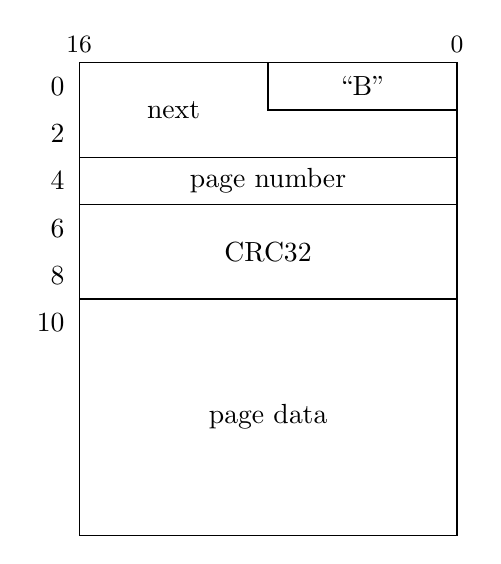
\begin{tikzpicture}[scale=0.3]
  \draw (0,0) rectangle (16,-20);
  \draw (8,0) -- (8,-2) -- (16,-2);
  \draw (0,-4) -- (16,-4);
  \draw (0,-6) -- (16,-6);
  \draw (0,-10) -- (16,-10);
%
  \node[anchor=east] at (-0.2,-1) {0};
  \node[anchor=east] at (-0.2,-3) {2};
  \node[anchor=east] at (-0.2,-5) {4};
  \node[anchor=east] at (-0.2,-7) {6};
  \node[anchor=east] at (-0.2,-9) {8};
  \node[anchor=east] at (-0.2,-11) {10};
  \node[anchor=south] at (0,0) {\small 16};
  \node[anchor=south] at (16,0) {\small 0};
%
  \node at (12,-1) {``B''};
  \node at (4,-2) {next};
  \node at (8,-5) {page number};
  \node at (8,-8) {CRC32};
  \node at (8,-15) {page data};
\end{tikzpicture}

The fields are defined as follows.

\begin{description}
  \item[``B''] Record type ID; ASCII character ``B,'' equal to 0x42.
  \item[next] Address of the next record, 24-bit little endian.  Lowest bit
    always zero because of word alignment, and upper seven bits always zero
    because of the 128K size of the SRAM.
  \item[page number] Page number to write.  This is technically the high
    byte of the program memory address for the start of the page, which must
    be aligned on a boundary of 1024 address units or 1536 bytes.  So the
    upper eight bits and the lower two bits of the 16-bit value in this
    field, are necessarily zero.  For example, to write the page starting at
    0x1400, the page number field contains 0x0014.
  \item[CRC32] The CRC32 value (parameters as used by Ethernet, ZModem, and
    so on) of the page data.
  \item[page data] The 1536 bytes that should be written to the specified
    page.
\end{description}

The code to handle this record type starts by calling
spi1\_finish\_transaction, a support routine that receives the bytes of the
record through SPI that were not already read by the main loop, and stores
them into the common data area.  Earlier in the source code, in the section
labelled ``Data memory,'' there were labels b\_record\_page, b\_record\_crc,
and b\_record\_data defined to ease access to the different fields in this
record.

Next, it checks the CRC32.  It calls the support routine start\_crc to
initialize the hardware, then runs a loop to call crc\_w0\_word for each
word of the page data.  Finally, it calls check\_crc\_result to verify that
the value in the record matches what the CRC32 hardware calculated.  Getting
good results from the CRC32 hardware is a little tricky, but the details of
that are encapsulated in the support routines.  If the CRC32 does not match,
then check\_crc\_result does not return; instead, it jumps to the failure
display, ending the loading process.

It is preferable to avoid any unnecessary writes to the flash program
memory, both to reduce wear and because writes take a relatively long time,
which is better to avoid for speed reasons.  So there is a further check to
see whether the data that would be written happens to match what is already
there.  This might be a common occurrence if someone tries ``updating'' a
module with the same firmware it already contains, or with a version close
to the existing one that may happen to contain identical bytes in some
places.  The loop starting at brec\_compare\_loop checks each byte of the
destination page in program memory against the proposed new data in RAM.  If
it detects no differences, then this is not an error, but the write for this
page should not proceed; in such a case the code just jumps back to
loader\_entry to read the next loader record, skipping further processing on
the current one.

If at least one byte does differ between the existing program memory and the
new data, then it will be necessary to erase and rewrite the page.  The code
sets up the flash SFRs for a page erase and calls perform\_flash\_operation
to pull the trigger.  Then it does the write, which is conducted one row (of
64 instructions, making eight rows in the page) at a time.  For each row, it
checks whether the entire row consists of instructions with the value
0xFFFFFF, which is the value that results from an erase operation.  If a row
of all 0xFFFFFF instructions is detected, then programming that row is
skipped (again, to reduce unecessary writes).

Once all eight rows have been checked and possibly rewritten, the code jumps
back to loader\_entry to handle the next loader record.

\section{C-record: do a CRC check}

The C-record requests a CRC check of a range of addresses in the SRAM.  It
is 16 bytes long, laid out like this.

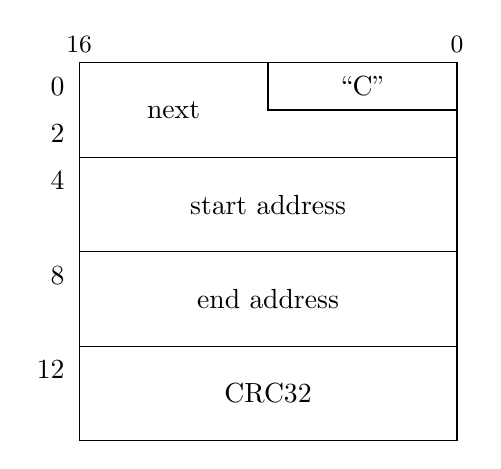
\begin{tikzpicture}[scale=0.3]
  \draw (0,0) rectangle (16,-16);
  \draw (8,0) -- (8,-2) -- (16,-2);
  \draw (0,-4) -- (16,-4);
  \draw (0,-8) -- (16,-8);
  \draw (0,-12) -- (16,-12);
%
  \node[anchor=east] at (-0.2,-1) {0};
  \node[anchor=east] at (-0.2,-3) {2};
  \node[anchor=east] at (-0.2,-5) {4};
  \node[anchor=east] at (-0.2,-9) {8};
  \node[anchor=east] at (-0.2,-13) {12};
  \node[anchor=south] at (0,0) {\small 16};
  \node[anchor=south] at (16,0) {\small 0};
%
  \node at (12,-1) {``C''};
  \node at (4,-2) {next};
  \node at (8,-6) {start address};
  \node at (8,-10) {end address};
  \node at (8,-14) {CRC32};
\end{tikzpicture}

The fields are defined as follows.

\begin{description}
  \item[``C''] Record type ID; ASCII character ``C,'' equal to 0x43.
  \item[next] Address of the next record, 24-bit little endian.  Lowest bit
    always zero because of word alignment, and upper 15 bits always zero
    because of the 128K size of the SRAM.
  \item[start address] Starting address of the range to check; 17-bit byte
    address stored as a 32-bit little endian unsigned integer, so the top 15
    bits are expected to be zero.
  \item[end address] Address of the first byte \emph{after} the range to
    be checked, as a 32-bit little endian unsigned integer; in consequence
    of that definition, end address minus start address equals number of
    bytes to check.
  \item[CRC32] The CRC32 value (parameters as used by Ethernet, ZModem, and
    so on) expected for the byte range.
\end{description}

The code for this record type starts by calling spi1\_finish\_transaction to
read the remaining 12 bytes of the record into the common data area.  Then,
it initializes the CRC32 hardware with a call to start\_crc, and starts a
READ transaction with the SRAM chip for the starting address of the range to
check.  It does a double-precision subtraction to find the byte count, and
runs a loop that reads that many bytes from the SPI port, sending each one
to the CRC32 hardware.  Finally, it calls check\_crc\_result to verify that
the value calculated by the hardware matches the one stored in the C-record. 
If the match fails, check\_crc\_result never returns; if it succeeds, the
C-record code ends with a branch to loader\_entry to handle the next loader
record.

Be aware that although a C-record can refer to any addresses in the SRAM, it
may be difficult or impossible to construct one that will succeed when the
range to be checked covers, overlaps, or contains bytes that depend on the
C-record's own CRC32 field.  Because of that and the fact that the range
must be a single interval, getting full coverage of the image file is a bit
tricky and requires multiple C-records.  See the discussion of image.s below
for how full coverage is achieved in the standard build.

\section{I-record: check hardware ID}

The I-record is intended to help make sure that a firmware image in this or
a similar format is really intended to be loaded on the hardware currently
trying to load it.  If at some point North Coast Synthesis were to release
other digital modules with a similar design, or if someone modified the
Gracious Host hardware in a way that would break the compatibility of
firmware images, then it would be important not to accidentally load a
firmware image intended for one of the hardware designs, on the other
hardware.  So to prevent problems in such a case, the hardware has a 64-bit
ID code, stored at the label HARDWARE\_ID at address 0xA800, in the first
eight bytes of the non-reprogrammable final page of program memory.  The
I-record specifies the intended hardware ID for the current image, and the
loader will abort if it sees an I-record that does not match the ID
of the current hardware platform.

The hardware ID for the Gracious Host, in the version described by this
manual (which as of this writing is the only version that exists), is 0x4D
0x53 0x4B 0x20 0x30 0x31 0x34 0x01.  That is the ASCII string ``MSK 014''
followed by a byte of value 0x01 which can be thought of as a version
number.

Please use a different hardware ID for any hardware that uses substantially
this image file format but is not 100\%\ compatible with firmware written
for the standard Gracious Host hardware.

The record layout is straightforward, just the common header shared by all
loader records, followed by the desired hardware ID.

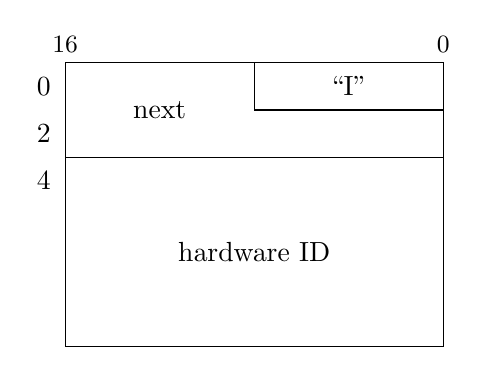
\begin{tikzpicture}[scale=0.3]
  \draw (0,0) rectangle (16,-12);
  \draw (8,0) -- (8,-2) -- (16,-2);
  \draw (0,-4) -- (16,-4);
%
  \node[anchor=east] at (-0.2,-1) {0};
  \node[anchor=east] at (-0.2,-3) {2};
  \node[anchor=east] at (-0.2,-5) {4};
  \node[anchor=south] at (0,0) {\small 16};
  \node[anchor=south] at (16,0) {\small 0};
%
  \node at (12,-1) {``I''};
  \node at (4,-2) {next};
  \node at (8,-8) {hardware ID};
\end{tikzpicture}

The fields are defined as follows.

\begin{description}
  \item[``I''] Record type ID; ASCII character ``I,'' equal to 0x49.
  \item[next] Address of the next record, 24-bit little endian.  Lowest bit
    always zero because of word alignment, and upper 15 bits always zero
    because of the 128K size of the SRAM.
  \item[hardware ID] The hardware ID to match against.
\end{description}

The code for this record type just loads the hardware ID from SRAM with a
call to spi1\_finish\_transaction, compares it against the one on the final
page of program memory, and branches to failure\_tune or loader\_entry
depending on the result of the comparison.

\section{J-record: jump to address}

The J-record tells the loader to jump (with a computed \insn{goto}
instruction) to a specified address in program memory.  This facility is
used midway through the loading process, after burning the high copy of the
loader, to transfer control to the new firmware's loader code instead of
depending on the low copy left behind by the old firmware.  It is also used,
at least in a standard firmware build, to start the calibration process
after loading is complete.

The record layout consists of the standard header, followed by the address
for the jump.

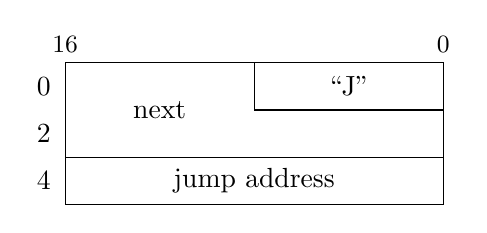
\begin{tikzpicture}[scale=0.3]
  \draw (0,0) rectangle (16,-6);
  \draw (8,0) -- (8,-2) -- (16,-2);
  \draw (0,-4) -- (16,-4);
%
  \node[anchor=east] at (-0.2,-1) {0};
  \node[anchor=east] at (-0.2,-3) {2};
  \node[anchor=east] at (-0.2,-5) {4};
  \node[anchor=south] at (0,0) {\small 16};
  \node[anchor=south] at (16,0) {\small 0};
%
  \node at (12,-1) {``J''};
  \node at (4,-2) {next};
  \node at (8,-5) {jump address};
\end{tikzpicture}

The fields are defined as follows.

\begin{description}
  \item[``J''] Record type ID; ASCII character ``J,'' equal to 0x4A.
  \item[next] Address of the next record, 24-bit little endian.  Lowest bit
    always zero because of word alignment, and upper 15 bits always zero
    because of the 128K size of the SRAM.  This is only used if loading
    continues after the jump; depending on where the jump is to, there may
    be no return from it.
  \item[jump address] Program memory address for the jump destination;
    16-bit little endian.
\end{description}

The code for this record just calls spi1\_read\_byte twice to get the jump
address, retracts CS2 to end the SPI transaction, and does the jump.

\section{S-record: succeed}

The S-record terminates the loader with a successful result.  As of this
writing, the standard firmware image does not actually use an S-record;
instead, when loading completes, it jumps to the calibration routine with a
J-record.  The image file contains an S-record at the end just in case
something causes the J-record to be skipped.  Successful calibration ends
with a jump to the global entry point SUCCESS\_TUNE, which calls
config\_timers\_for\_tunes and then branches into the S-record code, so this
code does in fact run after successful loading even though not invoked
through an S-record.

The only critical part of the S-record is the ``S'' at the start.

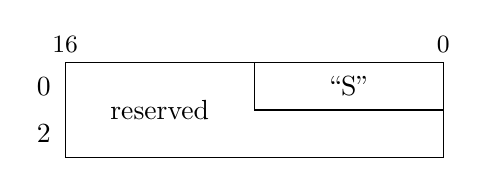
\begin{tikzpicture}[scale=0.3]
  \draw (0,0) rectangle (16,-4);
  \draw (8,0) -- (8,-2) -- (16,-2);
%
  \node[anchor=east] at (-0.2,-1) {0};
  \node[anchor=east] at (-0.2,-3) {2};
  \node[anchor=south] at (0,0) {\small 16};
  \node[anchor=south] at (16,0) {\small 0};
%
  \node at (12,-1) {``S''};
  \node at (4,-2) {reserved};
\end{tikzpicture}

The fields are defined as follows.

\begin{description}
  \item[``S''] Record type ID; ASCII character ``S,'' equal to 0x53.
  \item[reserved]  Although the S-record formally includes three bytes for
    the next-record pointer, these bytes are not actually used because
    executing an S-record terminates the loader.
\end{description}

The S-record code, starting from the label success\_tune, turns on the
front-panel LEDs and then runs 30 loops of playing a six-note tune that
takes two seconds to play, in square waves on the digital output jacks.  The
config\_timers\_for\_tunes subroutine will previously have set up output
compare peripheral number~1 (OC1) to be connected to those jacks and ready
to generate audio frequencies.

\includegraphics{success.cropped.eps}

Timing for the success display works using Timer~1, which has previously
been configured to 1:256 prescaler mode, 16\,$\mu$s per count.  At the start
of the loop the current value of the timer (TMR1 register) is captured into
W4.  Then at each step (for each note and the rest or pause at the end) code
in the support routine wait\_ticks computes a new target value for Timer~1
by adding an appropriate number to W4, and runs a tight loop that compares
TMR1 against the target value, terminating when they match exactly.  This
way there is no need for special handling of the timer overflow.  The loop
runs much faster than the 16\,$\mu$s counting rate of Timer~1, so it should
be unable to miss the exact match, especially bearing in mind that all
interrupts are turned off at this point.

In the success\_tune loop there are six calls to the support routine
play\_note, which sets OC1 to the period specified in W2 and then falls
through into wait\_ticks to wait 250\,ms, the duration of each note.  Then
the loop clears OC1R and OC1RS to make the output compare peripheral go
silent, and calls wait\_ticks with an argument value that makes it wait
500\,ms, for the rest at the end of the tune.

After 30 loops of the success tune, a \insn{reset} instruction reboots the
module.

Maintenance code 4935 invokes the success display.  See the discussion of
maintenance codes in the typing-keyboard driver documentation.

\section{F-record: fail}

The F-record terminates the loader with an \emph{unsuccessful} result; it is
basically similar to the S-record, but with a different display intended to
convey the idea of a failed loading attempt.  As with the S-record, current
firmware images never actually include F-records directly, but this record
type exists for testing, possible future use, as a destination for other
code paths that need to report failures, and to make it likely that files
other than valid firmware images will terminate processing quickly and
harmlessly.

In principle, the F-record's corrent type ID is ASCII ``F,'' but any loader
record with a type ID not otherwise handled will be treated as an F-record.

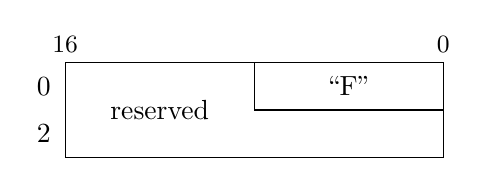
\begin{tikzpicture}[scale=0.3]
  \draw (0,0) rectangle (16,-4);
  \draw (8,0) -- (8,-2) -- (16,-2);
%
  \node[anchor=east] at (-0.2,-1) {0};
  \node[anchor=east] at (-0.2,-3) {2};
  \node[anchor=south] at (0,0) {\small 16};
  \node[anchor=south] at (16,0) {\small 0};
%
  \node at (12,-1) {``F''};
  \node at (4,-2) {reserved};
\end{tikzpicture}

The fields are defined as follows.

\begin{description}
  \item[``F''] Record type ID.  ASCII character ``F,'' equal to 0x46, is
    guaranteed to be treated as an F-record, but any value that is not the
    ID of some other record type will be treated as an F-record by default.
  \item[reserved]  Although the F-record formally includes three bytes for
    the next-record pointer, these bytes are not actually used because
    executing an F-record terminates the loader.
\end{description}

The code to handle F-records, starting from failure\_tune, is similar to
that for the success tune, but a little simpler because there are only four
notes, no rest, and the frequencies alternate between low B and other
pitches.

\includegraphics{failure.cropped.eps}

The play\_failure\_notes support routine plays two notes of 500\,ms each,
one low B and one other pitch specified by the period in W2, with the LEDs
turned off for the first note and on for the second.  The failure tune loop
is basically just two calls to play\_failure\_notes.  Before the loop, it
sets the colour of the front-panel LEDs to red.  After the loop, it executes
a \insn{reset} instruction to reboot the module.

The (capitalized) FAILURE\_TUNE global symbol is available for other code
paths to play the failure tune.  It just calls config\_timers\_for\_tunes to
set up the hardware and falls through into (uncapitalized, non-global)
failure\_tune.  FAILURE\_TUNE is conditionally assembled only in the low
copy of the loader, and its absence from the high copy is counted in
loader\_delta.

Maintenance code 6697 invokes the failure display.  See the discussion of
maintenance codes in the typing-keyboard driver documentation.

\section{Support routines}

The loader source file ends with a few support routines used by the code
above.  Several of these are also exposed as global symbols, only in the low
copy according to conditional assembly directives, because they are useful
elsewhere in the firmware.

The spi1\_read\_byte routine (also SPI1\_READ\_BYTE, used in the USB Mass
Storage driver) reads one byte from the SPI bus, either because we actually
want to read a byte, or to keep up the read/write balance needed to make
written bytes pass through the system.  The new byte goes into the low byte
of W0, and the previous low byte of W0 is swapped into the high byte, which
is useful when reading a 16-bit number with two successive byte reads.

The spi1\_finish\_transaction routine is specific to the loader and not
globally exposed.  It takes a byte count in W5 and reads that many bytes
from SPI into data memory starting at the address in W4, with the assumption
that exactly two of those bytes have already been requested (so it makes
W5$-$2 requests for new bytes).  It also closes the SPI transaction assumed to
already be in progress.  Some per-record-type handlers use this to load the
rest of their record data after the header.

The success and failure tunes use play\_failure\_notes, play\_note, and
wait\_ticks, each already described.

Then there are several routines for dealing with the CRC hardware.  The
start\_crc routine (globally exposed as START\_CRC) sets up the SFRs for the
CRC32 peripheral to start a CRC calculation, telling it to use 8-bit data
transfers and a 32-bit polynomial size.  The polynomial, in the format
required, is set by the constant crc\_polynomial and equal to
$x^{32}+x^{26}+x^{23}+x^{22}+x^{16}+x^{12}+x^{11}+x^{10}+x^8+x^7+x^5+x^4+x^2+x+1$
(hex value 0x04C11DB7, with the 33rd bit omitted).  This code also sets the
peripheral's shift register value to the constant crc\_init, which is
0x46AF6449, the value needed to make the PIC24F's CRC32 peripheral match the
behaviour of the CRC32 algorithm which specifies 0xFFFFFFFF initialization.

I think, though this initialization value came mostly from trial and error
in the simulator rather than a deep understanding of how the hardware works,
that what is going on here is that 0x46AF6449 is the value that would end up
in the register if we started with zero and then hashed 0xFFFFFFFF on the
data input, which is equivalent to what the standard's somewhat different
representation would call starting with 0xFFFFFFFF in the first place.  This
surmise is supported by other tricky distinctions in the handling of the
final check at the end.  It appears that the PIC24F hardware may be in some
way inside-out relative to other descriptions of CRC32.  I was not able to
find good example code for this hardware that I could adapt for my purposes;
common wisdom among PIC24 programmers seems to be that the CRC32 peripheral
is just too complicated, and it is better to implement the algorithm in
software.

Proceeding with the hardware-based implementation, the crc\_w0\_word routine
(exposed globally as CRC\_W0\_WORD) accumulates a 16-bit value from W0,
\emph{little endian}, into the ongoing calculation by loading its two bytes
into the hardware FIFO and falling through into run\_crc.  That routine
(exposed globally as RUN\_CRC) triggers the hardware to start processing
bytes from the FIFO and then waits for it to empty the the FIFO.  Note that
the CRC32 hardware processes only one bit of input at a time, but runs at a
clock speed of twice the processor clock (therefore, 32\,MHz); so it runs
one byte per four instructions and the wait is unlikely to be significant. 
Although in principle the hardware is designed to allow the CRC32 to crunch
away while the processor is doing something else, adding buffer fill
juggling on top of the other complexities of using this hardware seems
unlikely to be worthwhile.

The final support routine for CRC calculation is check\_crc\_result.  It
works by running four data bytes from the address specified in W1 into the
CRC32 hardware as if they were additional data bytes, and then checking
whether the shift register contains 0xFFFFFFFF.  If the four bytes from [W1]
were the correct CRC32 value of the data processed before this point, then
the shift register should indeed end up containing 0xFFFFFFFF, indicating a
correct match.  In that case, check\_crc\_result returns.  Otherwise, it
branches to failure\_tune.

The last support routine in the source file is perform\_flash\_operation,
exposed as a global symbol PERFORM\_FLASH\_OPERATION with the addition of a
\insn{disi} instruction to temporarily disable interrupts, which is
unnecessary in internal calls because the loader runs with interrupts
globally disabled.  Apart from that wrinkle, this code is as specified in
the microcontroller data sheet.  Its function is to commence primary
ignition on a flash program memory operation, the details of the operation
having been previously specified by writes to various SFRs and
flash-specific write latches.  Because doing such a thing is dangerous, the
hardware requires very specific steps with precise timing to ``arm'' and
trigger the operation; otherwise, the request will be ignored.  After
triggering the flash operation, the code contains a tight loop which waits
for the hardware to indicate the operation is complete.  The data sheet says
that an erase requires 40\,ms minimum, and a write requires 3\,ms typical,
though I could not find a timing diagram or a clear explanation of whether
that refers to a row or a single-instruction write, or whether those two
kinds of writes may have the same duration.

At the end of loader.s, the loader\_end label captures the assembly location
counter at the end of the double-assembled section, for use by mkloaddr to
calculate the location of the high copy.

\section{Image generation overview}

The source file image.s generates the loadable image, using the assembler to
piece together the records with the proper link addresses and so on.  The
basic concept was that using the same toolchain that generates ordinary
object files would make it easy to do things like make a J-record point at
the address of its target.  Unfortunately, bugs and limitations in the
assembler and linker mean that much of the logic for building the image ends
up implemented in macros instead of directly using the
assembler features, and there are several pieces of support code that need
to be invoked by the Makefile to get information into and out of the image
generator.  It is less simple than originally intended; but it does work.

One limitation in particular is that, because the image file gets assembled
into an object section of ``customized data memory'' type, it is not treated
as code by the toolchain, and some of the toolchain features that would be
available in code sections are unavailable.  (Trying to make it code instead
raised other problems and proved unworkable.) In particular, I was unable to
attach a label to a point in the image file and then say ``These bytes right
here should be filled in with the address of that label.'' Filling in such
bytes would normally be a function performed by the linker, and the linker
refuses to touch customized data memory.  So I ended up having to perform
the ``bytes should be the address of label'' operation by writing my own
code to extract the addresses of symbols and then fill them into the image,
defeating one of the original purposes of using the assembler for image
generation.

Another assembler limitation is that customized data memory spaces cannot be
bigger than 64K, and addresses within them cannot be bigger than 16 bits. 
The SRAM is 128K, requiring 17-bit addresses.  I dealt with that limitation
by actually defining two customized data memory spaces (referred to in the
source code as the low and high \emph{mobies}), with some logic required to
handle switching between them where necessary.  In practice, firmware is
unlikely to grow so big as to require the use of both; but in principle,
program memory is slightly greater than 64K all by itself (because of the
weirdness arising from its 24-bit width); firmware could fill all of program
memory; and the overhead of packaging it in loader records could push the
image file further past the moby boundary.

The Makefile builds the firmware binary by first running the assembler to
generate object files (*.o) from the assembly-language source files (*.s). 
In general there is one object file for each source file, although as
discussed above, loader.s actually builds two object files, loader-lo.o and
loader-hi.o.  Then the linker runs to decide the final addresses of all the
sections of code and combine the object files into a single unified binary
file (firmware.elf) that represents the entire contents of program memory. 
This file is in ELF format, the same format that under Linux (since version
1.2, anyway) would be an executable file.  For ICSP purposes, the ELF file
can be translated to a .hex file, which is the format usually used by
chip-programming hardware tools; the Makefile includes a rule to do that if
desired.

However, to generate a file that can be loaded by the module itself over the
USB port, there are more steps needed.  The Makefile uses the toolchain's
objdump utility, piped into a Perl script named dmp2bin, to generate the
files firmware.bin (which is a plain image of the contents of program
memory, all 66048 bytes of it) and fw-pages.inc, which defines symbols with
names like \_\_page\_exists\_\_00 for all the pages that contain data and
will need to be programmed.  These files are used as inputs by image.s to
decide which pages need B-records and to provide the data bytes for those
B-records.

Another Makefile rule generates the file firmware.syms from firmware.elf by
running the toolchain's nm utility.  This file lists all the program memory
addresses of symbols in the firmware.

Two more include files needed by image.s are image-syms.inc, which includes
the CRC values of parts of the image file for use in C-records, as well as
the addresses of symbols jumped to by J-records; and image-id.inc, which
includes metadata about the current build:  the username, hostname, and date
as reported by Linux command-line utilities.  Both of these files are
generated inside the final firmware.frm Makefile rule.

The rule that finally generates firmware.frm is a shell script written into
the Makefile, that puts together all the pieces.  One of the problems to be
solved is that the image file needs to contain CRC32 values for parts of
itself.  In order to calculate those values and write the image file, we
must already have the image file, creating a problem of where to start.  The
solution is that the Makefile rule is a shell-script loop: it builds the
image file using dummy data for the CRC32 values, then calculates new CRC32
values based on the result, and re-generates the file using those values. 
It repeats until the firmware.frm file does not change between two
iterations.  The CRC32 values do not (at least, should not) actually depend
upon \emph{themselves} directly or indirectly, only upon \emph{other bytes
in the file}, so the process terminates after two or three iterations.

In more detail, the Makefile rule initializes firmware.frm to a zero-length
file and image-syms.inc to a file containing a single newline.  (Use your
imagination for why the newline is necessary.) It creates the file
image-id.inc using the whoami, hostname, and date commands.  Then it
assembles image.s.  The macros in image.s figure out everything that should
be in the loadable image, but because image-syms.inc defines no symbols, the
macros just use dummy values for all the CRC32s and J-record destinations. 
After this assembly step, the Makefile rule does some bookkeeping for Make's
dependency tracking, uses nm to generate image.syms, and uses dmp2bin to
generate a tentative firmware.frm file.  This first version will not
actually be usable because of the dummy CRC32 and J-record data.

Then the loop starts.  It runs a Perl script called mkimagesyms, which
generates the image-syms.inc file based on the information in the tentative
firmware.frm, and the firmware.syms and image.syms files.  The script does
several things, controlled by symbols that were defined in image.s.

\begin{itemize}
  \item If symbols named like \_\_crc\_start\_\_XXXX and \_\_crc\_end\_\_XXXX
    are defined, then mkimagesyms will compute the CRC32 of the bytes between those
    symbols in firmware.frm, and will define a symbol in image-syms.inc named
    like \_\_crc\_\_XXXX and equal to the CRC32 value.
  \item When it computes a CRC32 value, mkimagesyms will also define
    symbols in image-syms.inc named like \_\_crc\_addra\_\_XXXX and
    \_\_crc\_addrz\_\_XXXX and equal to the starting and ending addresses of
    the CRC32 calculation.  These differ from 
    \_\_crc\_start\_\_XXXX and \_\_crc\_end\_\_XXXX, despite normally having
    the same numerical values, because these new symbols have the
    data type of plain numbers, not address labels.  The assembler can set
    data bytes equal to them, which it would refuse
    to do with address labels.  They also are adjusted by the
    \emph{moby} feature below to contain the 17th address bit that the
    assembler refuses to handle.
  \item If a symbol named like \_\_moby\_\_XXXX is defined, then the value
    of that symbol times 0x10000 (that is, 64K) is added to the address of
    the symbol \_\_XXXX before \_\_XXXX is used for other purposes. 
    This facility would normally be used for CRC32 start
    and end addresses, with symbols named like
    \_\_moby\_\_crc\_start\_\_XXXX, to express which half of the 128K SRAM
    actually contains a given address.
  \item If a symbol named like \_\_psym\_\_XXXX is defined, then mkimagesyms
    will define that symbol in image-syms.inc to have the value of the
    \emph{program memory} address of the symbol XXXX in the firmware, taken
    from firmware.syms.  This is used for J-record targets.
  \item It detects whether the image-syms.inc file it is writing is
    identical to the one that previously existed, and returns a success exit
    code (exit code zero) if so.
\end{itemize}

Then the script runs the assembler on image.s again.  The image.s file
includes image-syms.inc, which now gives real (though perhaps not final)
values to the CRC32 and J-record values.  The script runs the steps to
regenerate image.syms and firmware.frm, then repeats until mkimagesyms
returns exit code zero.  It displays the sha1sum output for
image-syms.inc on each iteration, to give the user some idea that progress
is being made, although the actual check for loop termination is on exact
equality, not on the sha1sum result.

\section{The image generator source file (image.s)}

The source file image.s puts the pieces together.  It starts by including
global.inc (like all the firmware source files); fw-pages.inc (which
contains a symbol per page identifying the pages to burn); and
image-syms.inc (generated by mkimagesyms, as above).

Then it sets up a memory space for each 64K moby of the SRAM (spaces named
\_sram\_lo and \_sram\_hi), defines max\_record to 1546 to represent the
largest possible loader record (which is needed for detecting when to switch
mobies).  It opens an assembly section in \_sram\_lo, which will be the
destination for the image data; then it starts defining the support macros.

The basic flow is that we keep a shadow location counter in the symbol
\_\_location, which records where we are currently assembling things into
the SRAM's space.  Keeping it in a symbol of our own is necessary because
the assembler narrowly limits the ways we can use the value of its own
location counter.  As we create loader records with the macros defined for
the purpose, this symbol gets updated to reflect where the next record will
be created.  When it is detected that the next record will not fit in the
current moby (or \emph{may} not fit -- the check is based on the assumption
of a maximum-length record), the macros automatically close the low moby
section and start assembling into a new section for the high moby.

The check\_moby macro comes first.  It just checks whether \_\_location plus
the maximum record size would exceed 64K, and if so, switches to a new
section.  This needs to be a separate macro because of an assembler bug:  if
we start a new section inside a macro and assemble bytes into that section
inside the same macro then the listing file is messed up.

So the loader\_record macro, which assembles the start of a loader record
(type ID and next-record link), is a separate macro, and the main source
code normally runs check\_moby before each invocation of loader\_record. 
The loader\_record macro takes as arguments the record type (one ASCII
character), a name used for defining a symbol associated with this record,
and the record's size in bytes.  The address of the next record is
calculated using this size, with appropriate adjustment for whether the next
record is being moved into the next moby.

The first 0x0100 bytes of the file contain an ASCII copyright notice and
version identifier.  The image-id.inc file gets included here so that the
firmware file will be automatically stamped with basic metadata.

Loader records start at address 0x0100.  The first is an I-record, requiring
the hardware ID to match the Gracious Host's.  Then come two C-records which
together cover the entire file.  There is a macro called store\_crc defined,
which takes a name like XXXX as an argument and checks whether the symbol
\_\_crc\_\_XXXX is defined.  If it is (because it came from image-syms.inc),
it assembles four bytes containing the symbol value.  If not, it defines the
symbol to the value 0xDEADBEEF, which will trigger mkimagesyms to generate a
proper value for it on the next iteration, and assembles bytes with that
value instead.  This macro is also used by the page-burning records later.

The two C-records interlock to cover the entire file.  The first one,
referred to as the ``hi'' C-record, covers everything after the CRC field of
the ``lo'' C-record, which is next.  The ``lo'' record covers everything
before its own CRC field, including the entirety of the ``hi'' record.  This
arrangment guarantees that every byte of the file either is covered by some
CRC, or is part of a CRC field, without any circular dependencies.  Any file
corruption in the class of errors detectable by the CRC32 algorithm will
result in at least one of these two checks failing.  For greater certainty,
the B-records also have CRC checks of their own.

The B-records are next.  There is a macro named burn\_page defined, whose
function is first to check whether a symbol named like
\_\_page\_exists\_\_00 has been defined.  If so, that indicates the
page in question needs to be included in the firmware image.  It sets up a
header for a B-record; calls store\_crc to either assemble the data bytes
for the CRC of the page (if they have been defined) or else assemble
0xDEADBEEF and define the symbols that request calculation of this CRC; and
then includes the appropriate 1536 bytes from firmware.bin with an
``.incbin'' directive.

The source file calls burn\_page for each page from 0xA4 down to 0x50 in
descending order, using the assembler's ``.irpc'' looping construct to
abbreviate the loop.  That will program roughly the top half of program
memory, for the pages actually defined in the firmware.  At this point
loader records are still being interpreted by the old firmware's low loader
copy.  But after page 0x50, there is a J-record pointing at
LOADER\_HI\_ENTRY, with the address for that retrieved by mkimagesyms
through the \_\_psym\_\_ feature.  This directs the old firmware's loader to
jump to the high copy of the new firmware's loader, which ought to have been
in the pages just burned.  Subsequent loader records are actually executed
by the new firmware's loader.

There follows another .irpc loop to burn all defined pages from 0x4C down to
0x00.  After that, firmware update will be complete.  The image file source
assembles another J-record to jump to CALIBRATION\_PROCEDURE, which should
terminate loader processing.  But it also assembles a final S-record as a
backstop.
